\documentclass[12pt]{article}
\usepackage[spanish]{babel}
\usepackage{apacite}
\usepackage[utf8]{inputenc}
\usepackage{amsmath}
\usepackage{cancel}
\usepackage{newtxtext,newtxmath}
\usepackage{listings}
\usepackage[usenames]{color}
\definecolor{gray97}{gray}{.97}
\definecolor{gray75}{gray}{.75}
\definecolor{gray45}{gray}{.45}
\definecolor{azul1}{RGB}{141,198,163}
\definecolor{azul2}{RGB}{24,107,122}
\definecolor{verde1}{RGB}{44,186,34}
\usepackage{textcomp}
\lstset{
        frame=Ltb,
        framerule=1pt,
        framextopmargin=3pt,
        framexbottommargin=3pt,
        framexleftmargin=0.4cm,
        framesep=0pt,
        rulesep=.4pt,
		backgroundcolor=\color{gray97},
		rulesepcolor=,
        tabsize=4,
        rulecolor=\color[RGB]{106, 182, 217}, %AZUL
        upquote=true,
        aboveskip={1.5\baselineskip}, %despues de la linea de texto
        columns=fixed,
        showstringspaces=false,
        extendedchars=true,
        breaklines=true,
        prebreak = \raisebox{0ex}[0ex][0ex]{\ensuremath{\hookleftarrow}},
        showtabs=false,
        showspaces=false,
        showstringspaces=false,
        basicstyle=\scriptsize\ttfamily\color[RGB]{39, 100, 46}, %Numeros de lineas, simbolos, puntos y coma y demas
        identifierstyle=\ttfamily\color[RGB]{56, 140, 189}, %variables
        commentstyle=\color[RGB]{62, 179, 101}, %comentarios
        stringstyle=\color[RGB]{247, 165, 42}, %impresiones
        keywordstyle=\bfseries\color[RGB]{237, 118, 150}, %funciones
        %
		numbers=left,
		numbersep=5pt,
		numberstyle=\tiny,
		numberfirstline = false,
		breaklines=true,
        }
\usepackage{graphicx}
\usepackage[colorinlistoftodos]{todonotes}
\usepackage{natbib} %citas bibliograficas estilo APA :p
\usepackage{eso-pic}
\usepackage{avant}
\usepackage[top=2cm,bottom=2cm,left=2.5cm,right=3cm,headsep=8pt,a4paper]{geometry}
\usepackage{fancyhdr}
\pagestyle{fancy}
\fancyhf{}
%\fancyhead[LE,RO]{}
\fancyhead[RE,LO]{Robótica}
\fancyfoot[CE,CO]{\leftmark}
\fancyfoot[LE,RO]{\thepage}
\renewcommand{\headrulewidth}{2pt}
\renewcommand{\footrulewidth}{1pt}
\usepackage{tabu}
\usepackage{array}
\usepackage{multirow}
\usepackage{amssymb}
\usepackage{makeidx}
\graphicspath{ {images/} }
\usepackage{wrapfig}
\usepackage{enumerate}
\usepackage{amsmath,tikz}
\usetikzlibrary{matrix}
\usepackage{steinmetz}
\newcommand*{\horzbar}{\rule[0.05ex]{2.5ex}{0.5pt}}
\usepackage{calc}
\usepackage{hyperref}
\date{\today}


\begin{document}

\begin{titlepage}
\newcommand{\HRule}{\rule{\linewidth}{0.5mm}} 
\center
\textsc{\LARGE  Benemérita Universidad \\[0.2cm] Autónoma de Puebla}\\[1.5cm] 

\includegraphics[width=4cm]{IMAGENES/escudo}\\[1cm]
\textsc{\Large Facultad de Ciencias de la Electrónica}\\[0.5cm] 
\textsc{\large Licenciatura en Electrónica}\\[0.5cm]
\HRule \\[0.4cm]
{ \huge \bfseries Dinámica y Control de Posición}\\[0.4cm] 
\HRule \\[1.5cm]
\begin{minipage}{\textwidth}
\center 
\textsc{\LARGE Robótica}\\[1.7cm] 
\emph{Profesor:} \\
Dr. Fernando Reyes Cortés \\[1cm]
\begin{tabular}{ll}
\emph{Alumno:} & \emph{Número de Matrícula:}\\
Hanan Ronaldo Quispe Condori  & 555010653\\
\end{tabular}
\end{minipage}\\[2cm]
\today
\end{titlepage}

\newpage
\section{Resumen}
En el presente reporte se trabajarán aspectos importantes del algoritmo de control propuesto, primeramente, se considerará el caso general de un robot manipulador de n grados de libertad y luego la explicación cualitativa de este algoritmo aplicado a un robot manipulador de dos grados de libertad,con esta finalidad, se obtendrá la ecuación en lazo cerrado usando el modelo dinámico del robot de n grados de libertad y se procederá a demostrar la existencia del punto de equilibrio, seguidamente se propondrá una función candidata de Lyapunov analizando que esta, sea una función definida positiva, despues, se demostrará la estabilidad de este punto. Ademas de esto, se demostrará que la componente de regulación de este algoritmo de control se encuentra acotada. Finalmente se hará la simulación en MATLAB usando el modelo dinámico de un robot manipulador de dos grados de libertad y el valor numérico de los parametros físicos proporcionados.
\newpage
\section{Propósitos}
\begin{itemize}
    \item Competencias Profesionales
    \begin{itemize}
        \item Analizar un esquema de control nuevo usando los conocimientos adquiridos durante todo el curso teniendo en cuenta las condiciones propuestas para esta tarea.
        \item Aplicar las tecnicas de simulación en MATLAB aprendidas para el análisis de algoritmos de control nuevos.
    \end{itemize}
    \item Competencias Generales
    \begin{itemize}
        \item Aplicar el razonamiento lógico matemático a la demostración de esquemas de control usando los contenidos teoricos desarrollados.
        \item Usar las habilidades de aprendizaje autónomo en la simulación en software de sistemas no lineales  autónomos. 
    \end{itemize}
\end{itemize}
\newpage
\section{Introducción}

En robótica el uso de ecuaciones diferenciales es vital dada la complejidad de los sistemas, un modelo dinámico expresado por estas ecuaciones nos permite explicar todos los fenomenos físicos que se encuentran en su estructura mecánica, dentro de estos fenomenos podemos mencionar.
\begin{itemize}
    \item Fuerzas Centrípetas y Coriolis
    \item Efectos Inerciales
    \item Par Gravitacional
\end{itemize}

Este modelo se obtiene usando la metodología de Euler-Lagrange, para la cual se obtiene el lagrangiano del robot manipulador $\mathcal{L}(q,\dot{q})=\mathcal{K}(q,\dot{q})-\mathcal{U}(q,\dot{q})$ siendo resultante el modelo dinámico para un robot manipulador de n grados de libertad formado por eslabones rígidos conectados por articulaciones libres de elasticidad en cadena cinemática abierta.

\begin{equation}
    \begin{split}
        \tau&=M(q)\ddot{q}+C(q,\dot{q})\dot{q}+g(q)+f_f(\dot{q},f_e)\\
    \end{split}
    \label{eq:n_gld}
\end{equation}

Este modelo se puede usar para propositos de simulación, diseño, contrucción del sistema mecánico, analisis y diseño de sistemas de control[\cite{reyes2011robotica}]. 

En continuación con esta temática se verá tambien el problema de regulación o control de posición, consiste en mover el extremo final del robot manipulador desde cualquier posición inicial $q(0)$ hacia una posición deseada $q_d$, con esta finalidad, se determinará una ley de control $\tau$ que proporcione los pares aplicados a los servomotores del robot, de tal forma que el error de posición del robot $\tilde{q}(t)$ y la velocidad articular $\dot{q}(t)$ convergan asintóticamente a cero sin importar las condiciones iniciales $\tilde{q}(0)$ y $\dot{q}(0)$ expresado matemáticamente esto se tendrá.

\begin{equation}
    \begin{split}
        \lim_{t\rightarrow\infty}
        \begin{bmatrix}
            \dot{q}(t)\\
            \tilde{q}(t)
        \end{bmatrix}&=
        \begin{bmatrix}
            0\\
            0
        \end{bmatrix}\\
    \end{split}
    \label{eq:lim_cerrado}
\end{equation}

Para determinar la ley de control $\tau$ recurriremos al enfoque de moldeo de energia, este permite diseñar una familia extensa de esquemas de control. Un esquema de control de posición es una ecuación cuya principal característica es  que genera un atractor en la ecuación de lazo cerrado formada por el modelo dinámico del robot manipulador y la estructura matemática del esquema de control. Lo que quiere decir que el atractor de las variables de estado corresponde al origen visto en un diagrama fase y por tanto dicho punto sea asintóticamente estable, esto hara que la influencia de las condiciones iniciales sea nula, el robot manipulador siempre llegara a la posición deseada $q_d$[\cite{reyes2011robotica}]. 

\begin{equation}
    \begin{split}
        \tau&=\nabla\mathcal{U}_a(K_p,\tilde{q})-f_v(K_v,\dot{q})+g(q)\\
    \end{split}
    \label{eq:moldeo}
\end{equation}

En la ecuación \ref{eq:moldeo} el término que se diseñará es $\mathcal{U}_a(K_p,\tilde{q})$ el cual corresponde a la energia potencial artificial, este diseño se llevará a cabo proponiendo una función de Lyapunov que tendrá la siguiente forma.

\begin{equation}
    \begin{split}
        V(\dot{q},\tilde{q})&=\frac{1}{2}\dot{q}^TM(q)\dot{q}+\mathcal{U}_a(K_p,\tilde{q})\\
    \end{split}
    \label{eq:energy}
\end{equation}

\section{Planteamiento y Descripción del Problema}
Considere el siguiente algoritmo de control:
\begin{equation}
    \begin{split}
        \tau&=K_p
        \begin{bmatrix}
            \frac{1}{cosh^2(\tilde{q})}\frac{tanh(\tilde{q})}{1+tanh^2(\tilde{q})}
        \end{bmatrix}
        -K_vatan(\dot{q})+g(q)
    \end{split}
    \label{eq:tau}
\end{equation}
Donde $K_p$,$K_v$ $\in \mathbb{R}^{n\times n}$ son matrices definidas positivas; además:
\begin{equation}
    \begin{split}
        \begin{bmatrix}
            \frac{1}{cosh^2(\tilde{q})}\frac{tanh(\tilde{q})}{1+tanh^2(\tilde{q})}
        \end{bmatrix}&=
        \begin{bmatrix}
            \frac{1}{cosh^2(\tilde{q_1})}\frac{tanh(\tilde{q_1})}{1+tanh^2(\tilde{q_1})}\\
            \frac{1}{cosh^2(\tilde{q_2})}\frac{tanh(\tilde{q_2})}{1+tanh^2(\tilde{q_2})}\\
            \vdots\\
            \frac{1}{cosh^2(\tilde{q_n})}\frac{tanh(\tilde{q_n})}{1+tanh^2(\tilde{q_n})}
        \end{bmatrix}
        \quad\text{y}\quad
        atan(\dot{q})=
        \begin{bmatrix}
            atan(\dot{q_1})\\
            atan(\dot{q}_2)\\
            \vdots\\
            atan(\dot{q_n})
        \end{bmatrix}\\
    \end{split}
    \label{eq:matrix_form}
\end{equation}
\begin{enumerate}
    \item Desmostrar la existencia y unicidad del punto de equilibrio de la ecuación en lazo cerrado.
    \item Proponer una función candidata de Lyapunov (demostrar analíticamente que dicha función se definida positiva).
    \item Demostrar la estabilidad del punto de equilibrio.
    \item Demostrar que la componente de regulación de (\ref{eq:tau}) se encuentra acotada.
    \item Realizar la simulación del algoritmo de control (\ref{eq:tau}) con el modelo dinámico numérico de un robot de 2 gld, tomando en cuenta las siguientes referencias:$\begin{bmatrix}
        q_{d1},&q_{d2}
    \end{bmatrix}^T=
    \begin{bmatrix}
    90^{\circ},&90^{\circ}
    \end{bmatrix}^T$. Considere un tiempo de simulación de $t=0$ a $10$ segundos y un periodo de muestreo $h=2.5mseg$. Explicar cualitativamente el funcionamiento del algoritmo de control(\ref{eq:tau}).
    \item Proponga una regla de sintonía de las ganancias proporcional $K_p\in \mathbb{R}^{2\times 2}$ y derivativa $K_v\in \mathbb{R}^{2\times 2}$, tal que la ley de control $\tau\in \mathbb{R}^{2\times 2}$ no rebase el torque del hombro $\tau^{max}_{1}=150Nm$ y para la articulación del codo $\tau^{max}_{2}=15Nm$. Grafique los pares aplicados y errores de posición.
\end{enumerate}
\section{Solución del Problema}
\begin{enumerate}
    \item Se procederá a armar la ecuación lazo cerrado, usando el modelo dinámico sin considerar la fricción de Coulomb ni la fricción estática de articulación y el algoritmo de control .
    \begin{equation}
        \begin{split}
            M(q)\ddot{q}+C(q,\dot{q})\dot{q}+g(q)+B\dot{q}&=K_p
            \begin{bmatrix}
                \frac{1}{cosh^2(\tilde{q})}\frac{tanh(\tilde{q})}{1+tanh^2(\tilde{q})}
            \end{bmatrix}
            -K_vatan(\dot{q})+g(q)\\
            M(q)\ddot{q}+C(q,\dot{q})\dot{q}+\cancel{g(q)}+B\dot{q}&=K_p
            \begin{bmatrix}
                \frac{1}{cosh^2(\tilde{q})}\frac{tanh(\tilde{q})}{1+tanh^2(\tilde{q})}
            \end{bmatrix}
            -K_vatan(\dot{q})+\cancel{g(q)}\\
            M(q)\ddot{q}+C(q,\dot{q})\dot{q}+B\dot{q}&=K_p
            \begin{bmatrix}
                \frac{1}{cosh^2(\tilde{q})}\frac{tanh(\tilde{q})}{1+tanh^2(\tilde{q})}
            \end{bmatrix}
            -K_vatan(\dot{q})
        \end{split}
        \label{eq:closed_loop}
    \end{equation}
    Despejando $\ddot{q}$ se tendrá
    \begin{equation}
        \begin{split}
            \ddot{q}&=M^{-1}(q)\lbrack K_p
            \begin{bmatrix}
                \frac{1}{cosh^2(\tilde{q})}\frac{tanh(\tilde{q})}{1+tanh^2(\tilde{q})}
            \end{bmatrix}
            -K_vatan(\dot{q})-C(q,\dot{q})\dot{q}-B\dot{q}\rbrack
        \end{split}
        \label{eq:state}
    \end{equation}
    El error estara dado por la siguiente ecuación.
    \begin{equation}
        \begin{split}
            \tilde{q}&=q_d-q\\
            \dot{\tilde{q}}&=-\dot{q}\\
        \end{split}
        \label{eq:error}
    \end{equation}
    De las ecuaciones (\ref{eq:state}) y (\ref{eq:error}) se tendrá la ecuación en lazo cerrado.
    \begin{equation}
        \begin{split}
            \frac{d}{dt}\begin{bmatrix}
                \tilde{q}\\
                \dot{q}
            \end{bmatrix}=\begin{bmatrix}
                -\dot{q}\\
                M^{-1}(q)\lbrack K_p
            \begin{bmatrix}
                \frac{1}{cosh^2(\tilde{q})}\frac{tanh(\tilde{q})}{1+tanh^2(\tilde{q})}
            \end{bmatrix}
            -K_vatan(\dot{q})-C(q,\dot{q})\dot{q}-B\dot{q}\rbrack
            \end{bmatrix}
        \end{split}
        \label{eq:closed_matrix}
    \end{equation}
    La demostración de existencia y unicidad del punto de equilibrio$\begin{bmatrix}
        0,&0
    \end{bmatrix}^T \in  \mathbb{R}^{2n} $ será.
    \begin{equation}
        \begin{split}
            \frac{d}{dt}\begin{bmatrix}
                \tilde{q}\\
                \dot{q}
            \end{bmatrix}=\begin{bmatrix}
                -\dot{q}\\
                M^{-1}(q)\lbrack K_p
            \begin{bmatrix}
                \frac{1}{cosh^2(\tilde{q})}\frac{tanh(\tilde{q})}{1+tanh^2(\tilde{q})}
            \end{bmatrix}
            -K_vatan(\dot{q})-C(q,\dot{q})\dot{q}-B\dot{q}\rbrack
            \end{bmatrix}=\begin{bmatrix}
                0\\
                0
            \end{bmatrix}
        \end{split}
        \label{eq:demonstration}
    \end{equation}
    \begin{itemize}
        \item El primer término de la ecuación (\ref{eq:demonstration}) satisface $-\dot{q}=-I\dot{q}\leftrightarrow \dot{q}=0$ esto ya que $I \in \mathbb{R}^{n\times n}$ es la matriz identidad.
        \item Para el segundo término de la ecuación (\ref{eq:demonstration}) se tiene que $M(q)>0$
        por propiedad de ser definida positiva $M^{-1}(q)$ será tambien definida positiva, entonces para que se cumpla la condición $M^{-1}(q)\lbrack K_p
        \begin{bmatrix}
            \frac{1}{cosh^2(\tilde{q})}\frac{tanh(\tilde{q})}{1+tanh^2(\tilde{q})}
        \end{bmatrix}
        -K_vatan(\dot{q})-C(q,\dot{q})\dot{q}-B\dot{q}\rbrack=0$, se debe cumplir que $\lbrack K_p
        \begin{bmatrix}
            \frac{1}{cosh^2(\tilde{q})}\frac{tanh(\tilde{q})}{1+tanh^2(\tilde{q})}
        \end{bmatrix}
        -K_vatan(\dot{q})-C(q,\dot{q})\dot{q}-B\dot{q}\rbrack=0$, analizando esta expresión
        \begin{equation}
            \begin{split}
                C(q,\dot{q})\dot{q}=0\leftrightarrow\dot{q}=0\enspace \text{,}\enspace 
                B\dot{q}=0\leftrightarrow\dot{q}=0\enspace \text{,}\enspace -K_vatan(\dot{q})=0\leftrightarrow atan(0)=0
            \end{split}
            \label{eq:conditions}
        \end{equation}
        El ultimo factor que falta analizar es $K_p
        \begin{bmatrix}
            \frac{1}{cosh^2(\tilde{q})}\frac{tanh(\tilde{q})}{1+tanh^2(\tilde{q})}
        \end{bmatrix}$, en esta expresion dado que $K_p$ es definida positiva entonces $\begin{bmatrix}
            \frac{1}{cosh^2(\tilde{q})}\frac{tanh(\tilde{q})}{1+tanh^2(\tilde{q})}
        \end{bmatrix}=0\leftrightarrow\tilde{q}=0$, si gráficamos esta función podremos ver el comportamiento acotado del regulador propuesto.

        \begin{figure}[h]
            \centering
            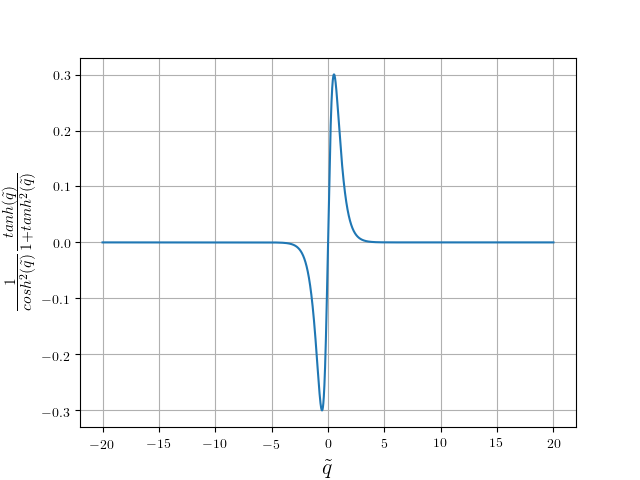
\includegraphics[width=12cm, height=7cm]{IMAGENES/tanh.png}
            \caption{Regulador Acotado.}
            \label{fig:regulador}
        \end{figure}

        Entonces podemos concluir que el punto $\lbrack\tilde{q},\dot{q} \rbrack=0\in\mathbb{R}^{2n}$ existe y es el único punto de equilibrio del sistema. 
    \end{itemize} 
    \item Se propondra la siguiente función candidata de Lyapunov compuesta por la suma de la energía cinética del robot manipulador y energia potencial artificial siguiendo la regla de diseño (\ref{eq:energy}).
    \begin{equation}
        \begin{split}
            V(\tilde{q},\dot{q})&=\frac{1}{2}\dot{q}^TM(q)\dot{q}+\frac{1}{2}
            \begin{bmatrix}
                \sqrt{ln(tanh^2(\tilde{q_1})+1)}\\
                \sqrt{ln(tanh^2(\tilde{q_2})+1)}\\
                \vdots\\
                \sqrt{ln(tanh^2(\tilde{q_n})+1)}
            \end{bmatrix}^T
            K_p
            \begin{bmatrix}
                \sqrt{ln(tanh^2(\tilde{q_1})+1)}\\
                \sqrt{ln(tanh^2(\tilde{q_2})+1)}\\
                \vdots\\
                \sqrt{ln(tanh^2(\tilde{q_n})+1)}
            \end{bmatrix}
        \end{split}
        \label{eq:candidate}
    \end{equation}
    Esta función candidata de Lyapunov debe ser definida positiva, lo cual se procederá a demostrar.
    \begin{itemize}
        \item El primer sumado $\frac{1}{2}\dot{q}^TM(q)\dot{q}$ se puede observar que tiene la forma $x^TPx$ el cual según el teorema de silvestrer [\cite{reyes}] será definida positiva si y solo si la matriz $P$ es definida positiva. En este caso por propiedad del modelo dinámico la matriz de inercia $M(q)$ es definida positiva.
        \item En el caso de la energia potencial artificial se puede observa que $\mathcal{U}_a(K_p,\tilde{q})=\mathcal{U}_a(K_p,0)=0$
        \begin{equation}
            \begin{split}
                \mathcal{U}_a(K_p,0)&=
                \frac{1}{2}
            \begin{bmatrix}
                \sqrt{ln(tanh^2(0)+1)}\\
                \sqrt{ln(tanh^2(0)+1)}\\
                \vdots\\
                \sqrt{ln(tanh^2(0)+1)}
            \end{bmatrix}^T
            K_p
            \begin{bmatrix}
                \sqrt{ln(tanh^2(0)+1)}\\
                \sqrt{ln(tanh^2(0)+1)}\\
                \vdots\\
                \sqrt{ln(tanh^2(0)+1)}
            \end{bmatrix}\\
            \mathcal{U}_a(K_p,0)&=
                \frac{1}{2}
            \begin{bmatrix}
                \sqrt{ln(1)}\\
                \sqrt{ln(1)}\\
                \vdots\\
                \sqrt{ln(1)}
            \end{bmatrix}^T
            K_p
            \begin{bmatrix}
                \sqrt{ln(1)}\\
                \sqrt{ln(1)}\\
                \vdots\\
                \sqrt{ln(1)}
            \end{bmatrix}\\
            \mathcal{U}_a(K_p,0)&=
                \frac{1}{2}
            \begin{bmatrix}
                0\\
                0\\
                \vdots\\
                0
            \end{bmatrix}^T
            K_p
            \begin{bmatrix}
                0\\
                0\\
                \vdots\\
                0
            \end{bmatrix}\\
            \mathcal{U}_a(K_p,0)&=0
            \end{split}
            \label{eq:prove}
        \end{equation}
        Tambien se puede observar que $\mathcal{U}_a(K_p,\tilde{q})>0$ si $\tilde{q}\not = 0$, se puede concluir que $\mathcal{U}_a(K_p,\tilde{q})$ es definida positiva local ya que $\exists \rho>0,\gamma>)0:0<\mathcal{U}_a(K_p,\tilde{q})<\gamma$, se sabe que la suma de funciones definidas positivas es otra función definida positiva por lo tanto.
        \begin{equation}
            \begin{split}
                \frac{1}{2}\dot{q}^TM(q)\dot{q}>0\quad\text{y}\quad \mathcal{U}_a(K_p,\tilde{q})&>0\quad \therefore \quad \frac{1}{2}\dot{q}^TM(q)\dot{q}+\mathcal{U}_a(K_p,\tilde{q})>0\\
                V(\tilde{q},\dot{q})&=\frac{1}{2}\dot{q}^TM(q)\dot{q}+\mathcal{U}_a(K_p,\tilde{q})>0
            \end{split}
            \label{eq:defined_positive}
        \end{equation}
    \end{itemize}
    \item Para demostrar la estabilidad del punto se equilibrio se procederá a derivar la ecuación (\ref{eq:candidate}) con respecto al tiempo para obtener la potencia.
    
    \begin{equation}
        \begin{split}
            \dot{V}(\tilde{q},\dot{q})&=\frac{d}{dt}\begin{bmatrix}
                \frac{1}{2}\dot{q}^TM(q)\dot{q}+\frac{1}{2}
            \begin{bmatrix}
                \sqrt{ln(tanh^2(\tilde{q_1})+1)}\\
                \sqrt{ln(tanh^2(\tilde{q_2})+1)}\\
                \vdots\\
                \sqrt{ln(tanh^2(\tilde{q_n})+1)}
            \end{bmatrix}^T
            K_p
            \begin{bmatrix}
                \sqrt{ln(tanh^2(\tilde{q_1})+1)}\\
                \sqrt{ln(tanh^2(\tilde{q_2})+1)}\\
                \vdots\\
                \sqrt{ln(tanh^2(\tilde{q_n})+1)}
            \end{bmatrix}
            \end{bmatrix}\\
            \dot{V}(\tilde{q},\dot{q})&=
            \frac{d}{dt}\begin{bmatrix}
                \frac{1}{2}\lbrack\dot{q}^TM(q)\dot{q}))\rbrack
            \end{bmatrix}
            +\frac{d}{dt}
            \begin{bmatrix}
                \frac{1}{2}
            \begin{bmatrix}
                \sqrt{ln(tanh^2(\tilde{q_1})+1)}\\
                \sqrt{ln(tanh^2(\tilde{q_2})+1)}\\
                \vdots\\
                \sqrt{ln(tanh^2(\tilde{q_n})+1)}
            \end{bmatrix}^T
            K_p
            \begin{bmatrix}
                \sqrt{ln(tanh^2(\tilde{q_1})+1)}\\
                \sqrt{ln(tanh^2(\tilde{q_2})+1)}\\
                \vdots\\
                \sqrt{ln(tanh^2(\tilde{q_n})+1)}
            \end{bmatrix}
            \end{bmatrix}\\
            \frac{d}{dt}
            \begin{bmatrix}
            \frac{1}{2}\lbrack\dot{q}^TM(q)\dot{q}\rbrack
            \end{bmatrix}&=\frac{1}{2}\lbrack\dot{q}^TM(q)\ddot{q}+\ddot{q}^TM(q)\dot{q}+\dot{q}^T\dot{M}(q)\dot{q}\rbrack\\
            \frac{d}{dt}
            \begin{bmatrix}
            \frac{1}{2}\lbrack\dot{q}^TM(q)\dot{q}\rbrack
            \end{bmatrix}&=\frac{1}{2}\lbrack\dot{q}^TM(q)\ddot{q}+\dot{q}^TM(q)\ddot{q}+\dot{q}^T\dot{M}(q)\dot{q}\rbrack\\
            \frac{d}{dt}
            \begin{bmatrix}
            \frac{1}{2}\lbrack\dot{q}^TM(q)\dot{q}\rbrack
            \end{bmatrix}&=\frac{1}{2}\lbrack2\dot{q}^TM(q)\ddot{q}+\dot{q}^T\dot{M}(q)\dot{q}\rbrack\\
            \frac{d}{dt}
            \begin{bmatrix}
            \frac{1}{2}\lbrack\dot{q}^TM(q)\dot{q}\rbrack
            \end{bmatrix}&=\dot{q}^TM(q)\ddot{q}+\frac{1}{2}\dot{q}^T\dot{M}(q)\dot{q}\\
        \end{split}
        \label{eq:derivative}
    \end{equation}

    \begin{equation}
        \begin{split}
            \frac{d}{dt}\mathcal{U}_a(K_p,\tilde{q})&=\frac{d}{dt}(\frac{1}{2}\begin{bmatrix}
                \sqrt{ln(tanh^2(\tilde{q})+1)}
            \end{bmatrix}^TK_p\begin{bmatrix}
                \sqrt{ln(tanh^2(\tilde{q})+1)}
            \end{bmatrix})\\
            \frac{d}{dt}\mathcal{U}_a(K_p,\tilde{q})&=\frac{1}{2}2\begin{bmatrix}
                \sqrt{ln(tanh^2(\tilde{q})+1)}
            \end{bmatrix}^TK_p\frac{d}{dt}\begin{bmatrix}
                \sqrt{ln(tanh^2(\tilde{q})+1)}
            \end{bmatrix}\\
            \frac{d}{dt}\mathcal{U}_a(K_p,\tilde{q})&=\frac{1}{2}2\begin{bmatrix}
                \sqrt{ln(tanh^2(\tilde{q})+1)}
            \end{bmatrix}^TK_p\begin{bmatrix}
                \frac{2tanh(\tilde{q})\dot{\tilde{q}}}{2\sqrt{ln(tanh^2(\tilde{q})+1)}(tanh^2(\tilde{q})+1)cosh^2(\tilde{q})}
            \end{bmatrix}\\
            \frac{d}{dt}\mathcal{U}_a(K_p,\tilde{q})&=\frac{1}{\cancel{2}}\cancel{2}\cancel{\begin{bmatrix}
                \sqrt{ln(tanh^2(\tilde{q})+1)}
            \end{bmatrix}}^TK_p\begin{bmatrix}
                \frac{\cancel{2}tanh(\tilde{q})}{\cancel{2}\cancel{\sqrt{ln(tanh^2(\tilde{q})+1)}}(tanh^2(\tilde{q})+1)cosh^2(\tilde{q})}
            \end{bmatrix}\dot{\tilde{q}}\\
            \frac{d}{dt}\mathcal{U}_a(K_p,\tilde{q})&=-
            \begin{bmatrix}
                \frac{tanh(\tilde{q})}{(tanh^2{(\tilde{q})}+1)cosh^2(\tilde{q})}
            \end{bmatrix}^TK_p\dot{q}\\
        \end{split}
        \label{eq:derivative_1}
    \end{equation}
    Usando las ecuaciones (\ref{eq:derivative}), (\ref{eq:derivative_1}) y (\ref{eq:demonstration})se tendrá
    \begin{equation}
        \begin{split}
            \dot{V}(\tilde{q},\dot{q})&=\dot{q}^TM(q)\ddot{q}+\frac{1}{2}\dot{q}^T\dot{M}(q)\dot{q}-
            \begin{bmatrix}
                \frac{tanh(\tilde{q})}{(tanh^2{(\tilde{q})}+1)cosh^2(\tilde{q})}
            \end{bmatrix}^TK_p\dot{q}\\
            \dot{V}(\tilde{q},\dot{q})&=\dot{q}^T\cancel{M(q)}\cancel{M^{-1}(q)}\lbrack K_p
            \begin{bmatrix}
                \frac{1}{cosh^2(\tilde{q})}\frac{tanh(\tilde{q})}{1+tanh^2(\tilde{q})}
            \end{bmatrix}
            -K_vatan(\dot{q})-C(q,\dot{q})\dot{q}-B\dot{q}\rbrack\\&+\frac{1}{2}\dot{q}^T\dot{M}(q)\dot{q}-\dot{q}^TK_p
            \begin{bmatrix}
                \frac{tanh(\tilde{q})}{(tanh^2{(\tilde{q})}+1)cosh^2(\tilde{q})}
            \end{bmatrix}\\
            \dot{V}(\tilde{q},\dot{q})&=\dot{q}^T\lbrack K_p
            \begin{bmatrix}
                \frac{1}{cosh^2(\tilde{q})}\frac{tanh(\tilde{q})}{1+tanh^2(\tilde{q})}
            \end{bmatrix}
            -K_vatan(\dot{q})-C(q,\dot{q})\dot{q}-B\dot{q}\rbrack\\&+\frac{1}{2}\dot{q}^T\dot{M}(q)\dot{q}-\dot{q}^TK_p
            \begin{bmatrix}
                \frac{tanh(\tilde{q})}{(tanh^2{(\tilde{q})}+1)cosh^2(\tilde{q})}
            \end{bmatrix}\\
            \dot{V}(\tilde{q},\dot{q})&=\cancel{\dot{q}^T K_p
            \begin{bmatrix}
                \frac{1}{cosh^2(\tilde{q})}\frac{tanh(\tilde{q})}{1+tanh^2(\tilde{q})}
            \end{bmatrix}}
            -\dot{q}^TK_vatan(\dot{q})-\dot{q}^TC(q,\dot{q})\dot{q}-\dot{q}^TB\dot{q}\\&+\frac{1}{2}\dot{q}^T\dot{M}(q)\dot{q}-\cancel{\dot{q}^TK_p
            \begin{bmatrix}
                \frac{tanh(\tilde{q})}{(tanh^2{(\tilde{q})}+1)cosh^2(\tilde{q})}
            \end{bmatrix}}\\
            \dot{V}(\tilde{q},\dot{q})&=-\dot{q}^TK_vatan(\dot{q})-\cancel{\dot{q}^TC(q,\dot{q})\dot{q}}-\dot{q}^TB\dot{q}+\cancel{\frac{1}{2}\dot{q}^T\dot{M}(q)\dot{q}}\\
            \dot{V}(\tilde{q},\dot{q})&=-\dot{q}^TK_vatan(\dot{q})-\dot{q}^TB\dot{q}\leq 0\\
        \end{split}
        \label{eq:power}
    \end{equation}
    De la ecuación (\ref{eq:power}) se puede afirmar que $\dot{V}(\tilde{q},\dot{q})$ es semidefinida negativa, por lo tanto queda demostrada la estabilidad del punto de equilibrio.
    \item Para esta demostración se analizará el comportamiento del vector $\begin{bmatrix}
        \frac{1}{cosh^2(\tilde{q})}\frac{tanh(\tilde{q})}{1+tanh^2(\tilde{q})}
    \end{bmatrix}$.

    \begin{equation}
        \begin{split}
            f(\tilde{q})&=\begin{bmatrix}
                \frac{1}{cosh^2(\tilde{q})}\frac{tanh(\tilde{q})}{1+tanh^2(\tilde{q})}
            \end{bmatrix}\\
            \frac{d}{d(\tilde{q})}f(\tilde{q})&=g(\tilde{q})\\
            \frac{d}{d(\tilde{q})}j(\tilde{q})&=-ag(\tilde{q})\\
        \end{split}
        \label{eq:upper_limit}
    \end{equation}

    Definimos una función decreciente $\frac{d}{d(\tilde{q})}j(\tilde{q})$ para encontrar una ODE.

    \begin{equation}
        \begin{split}
            \frac{d}{d(\tilde{q})}j(\tilde{q})&=-ag(\tilde{q})\\
            dj(\tilde{q})&=-ag(\tilde{q})d(\tilde{q})\\
            \cancel{\int} \cancel{d}j(\tilde{q})&=\int-ag(\tilde{q})d(\tilde{q})\\
            J(\tilde{q})-J(\tilde{q_0})&=-a\int g(\tilde{q})d(\tilde{q})\\
            J(\tilde{q_0})&=a\int g(\tilde{q})d(\tilde{q})+J(\tilde{q})\\
        \end{split}
        \label{eq:lower_limit}
    \end{equation}

    Por el colorario de los numeros reales $a,b,c\in \mathbb{R}\rightarrow \quad a=b+c\leftrightarrow a>b\land a>c$ en la ecuación (\ref{eq:lower_limit}) se tendrá.
    \begin{equation}
        \begin{split}
            J(\tilde{q_0})&>a\int g(\tilde{q})d(\tilde{q})\\
        \end{split}
        \label{eq:done}
    \end{equation}
    Reemplazando la ecuación (\ref{eq:upper_limit}) en (\ref{eq:done}) se puede afirmar.
    \begin{equation}
        \begin{split}
            J(\tilde{q_0})&>a\begin{bmatrix}
                \frac{1}{cosh^2(\tilde{q})}\frac{tanh(\tilde{q})}{1+tanh^2(\tilde{q})}
            \end{bmatrix}\\
            \frac{J(\tilde{q_0})}{a}&>\begin{bmatrix}
                \frac{1}{cosh^2(\tilde{q})}\frac{tanh(\tilde{q})}{1+tanh^2(\tilde{q})}
            \end{bmatrix}\\
        \end{split}
        \label{eq:donex2}
    \end{equation}
    De la ecuación (\ref{eq:donex2}) se puede concluir que la componente de regulación esta acotada, adicionalmente a esto se puede afirmar [\cite{reyes2019family}].
    \begin{equation}
        \begin{split}
            \begin{vmatrix}\begin{vmatrix}\begin{bmatrix}
                \frac{1}{cosh^2(\tilde{q_1})}\frac{tanh(\tilde{q_1})}{1+tanh^2(\tilde{q_1})}\\
                \frac{1}{cosh^2(\tilde{q_2})}\frac{tanh(\tilde{q_2})}{1+tanh^2(\tilde{q_2})}\\
                \vdots\\
                \frac{1}{cosh^2(\tilde{q_n})}\frac{tanh(\tilde{q_n})}{1+tanh^2(\tilde{q_n})}
            \end{bmatrix}\end{vmatrix}\end{vmatrix}&<\frac{J(\tilde{q_0})}{a}
        \end{split}
        \label{eq:euclidean}
    \end{equation}
    \item Se procederá a graficar las funciones que conforman el esquema de control propuesto en la ecuación (\ref{eq:tau}) para su análisis cualitativo, este esquema se usara en MATLAB para la simulación usando el modelo dinámico del robot de dos grados con los parametros numéricos proporcionados .
    
    \vspace{15mm}

    \begin{figure}[h]
        \centering
        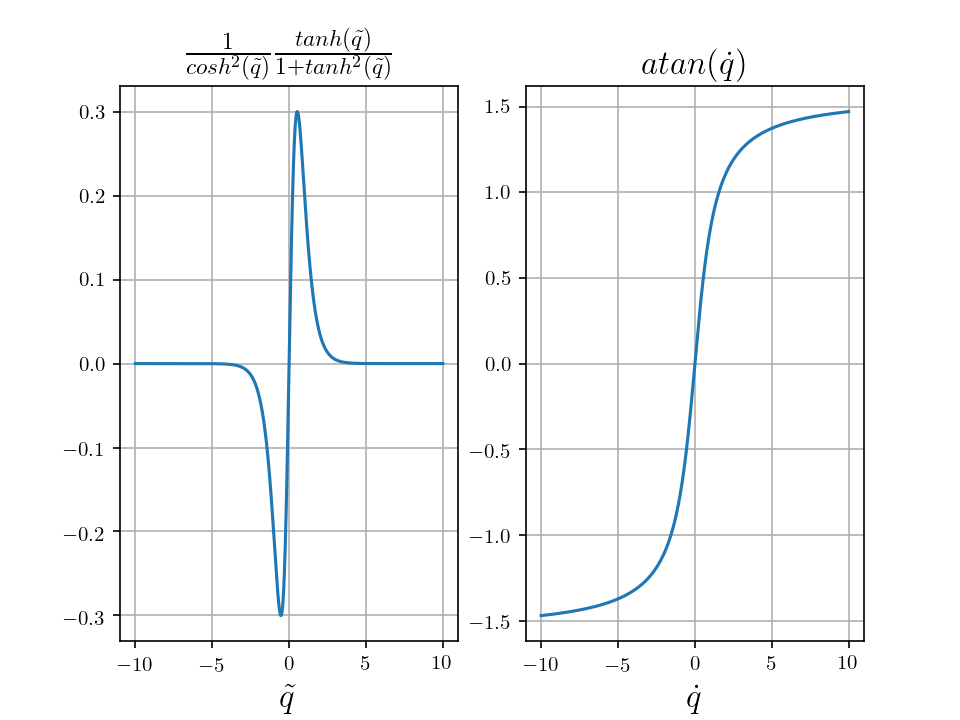
\includegraphics[width=14cm, height=6cm]{IMAGENES/comportamiento.png}
        \caption{Gráfica de Componentes del Esquema de Control.}
        \label{fig:comportamiento}
    \end{figure}
    
    Como se puede observar en las figuras ambas componentes se encuentran saturadas, para valores positivos muy grandes y negativos muy pequeños del error $\tilde{q}$, esta componente no tendrá efecto, en el caso de que $\tilde{q}$ sea pequeño o lo suficientemente grande, esta componente trabajará como un resorte no lineal de comportamiento hiperbólico. La componente $atan(\dot{q})$ producirá un efecto de amortiguamiento que atrapará los picos, sobreimpulsos de la repuesta transitoria para valores de $\dot{q}$ lo suficientemente grandes. 

    Para ejecutar la simulación se incluirán las siguientes lineas de código al archivo que contiene el algoritmo de control y la posición deseada $\begin{bmatrix}
        90^\circ,90^\circ
    \end{bmatrix}^T$.
    \lstinputlisting[language=matlab]{Matlab/tau.m}
    Al ejecutar la simulación se tendrán las siguientes gráficas de la posición y error de posición.
    \begin{figure}[h]
        \centering
        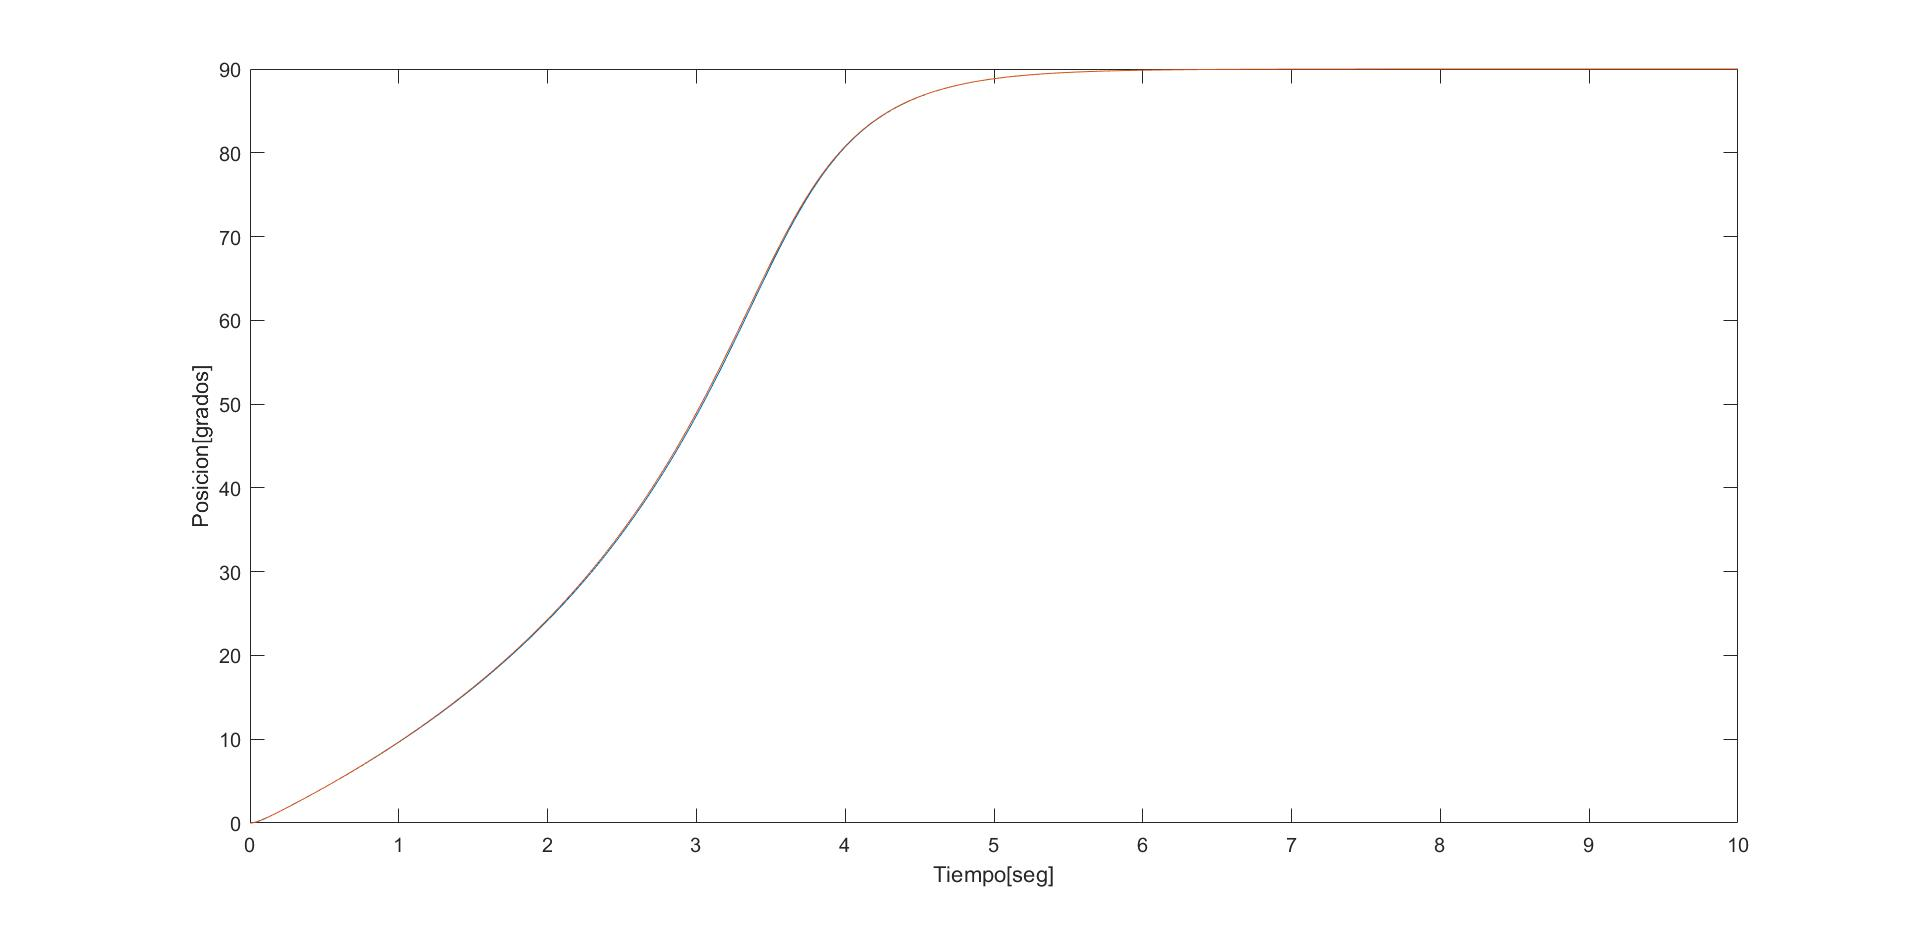
\includegraphics[width=14cm, height=6cm]{IMAGENES/pos.jpg}
        \caption{Evolución de la Posición en el Tiempo.}
        \label{fig:position}
    \end{figure}

    \begin{figure}[h]
        \centering
        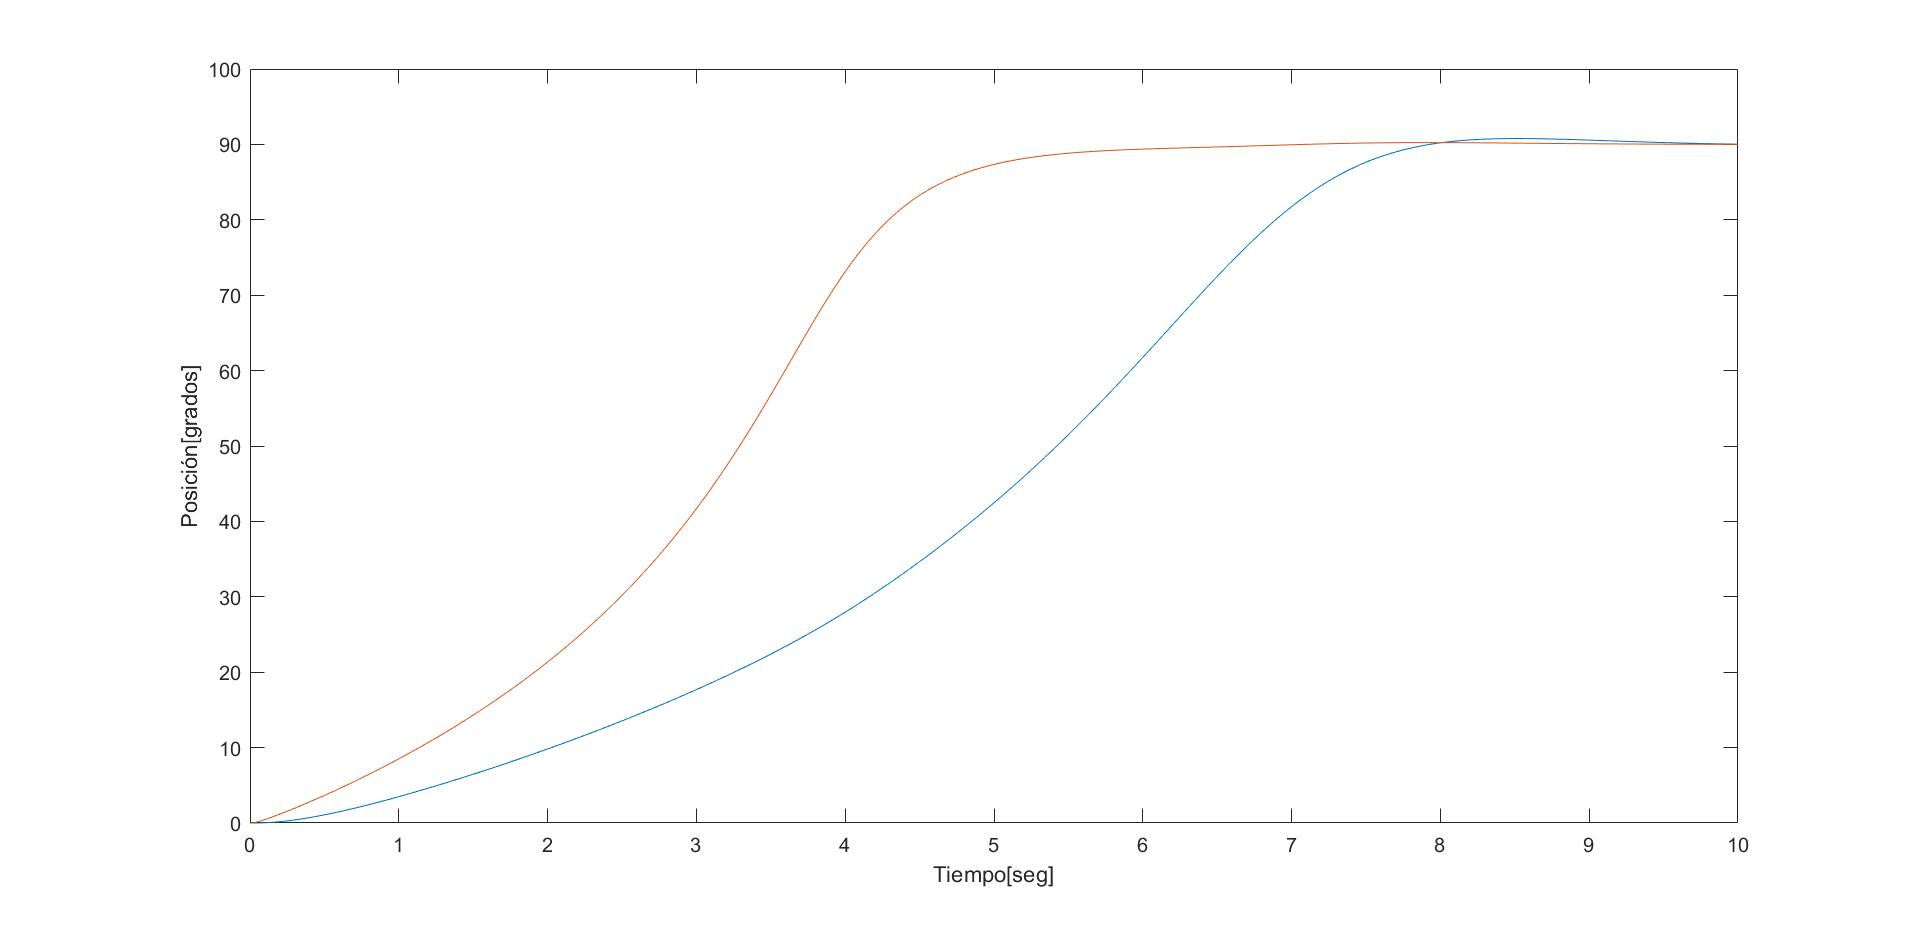
\includegraphics[width=14cm, height=6cm]{IMAGENES/pos1.jpg}
        \caption{Evolución de la Posición en el Tiempo, $K_p$ Disminuido.}
        \label{fig:position_1}
    \end{figure}

    En las figuras (\ref{fig:position}) y (\ref{fig:position_1}) se puede observar el efecto de las componentes de amortiguamiento y regulación del esquema de control, las curvas no presentan picos ni sobreimpulsos en su respuesta transitoria, en el caso de la figura (\ref{fig:position_1}) se disminuyo la ganancia $K_p$ con respecto a la figura (\ref{fig:position}) esto produjo un ligero sobreimpulso en la respuesta transitoria de la posición del codo, tambien se observa que el hombro alcanzo la posición deseada más rapido, ademas de ello, tanto el hombro como el codo llegan a $90^\circ$ suavemente esto debido a que el punto de equilibrio fue demostrado por lo que se tiene garantia que el algoritmo de control funciona antes de realizar la simulación.

    \item En el apartado anterior se vio que el esquema de control propuesto corresponde a un regulador saturado, por lo que la regla de sintonía por lo que se propondrá una función de la posición deseada y de los torques máximos para el hombro y codo del robot manipulador según una función hiperbólica.
    
    La regla de sintonía propuesta es la siguiente.
    \lstinputlisting[language=matlab]{Matlab/sintonia.m}
    
    Usando la regla de sintonía propuesta se procederá a gráficar los pares aplicados asi como errores de posición.
    %\vspace{50mm}
    \begin{figure}[h]
        \centering
        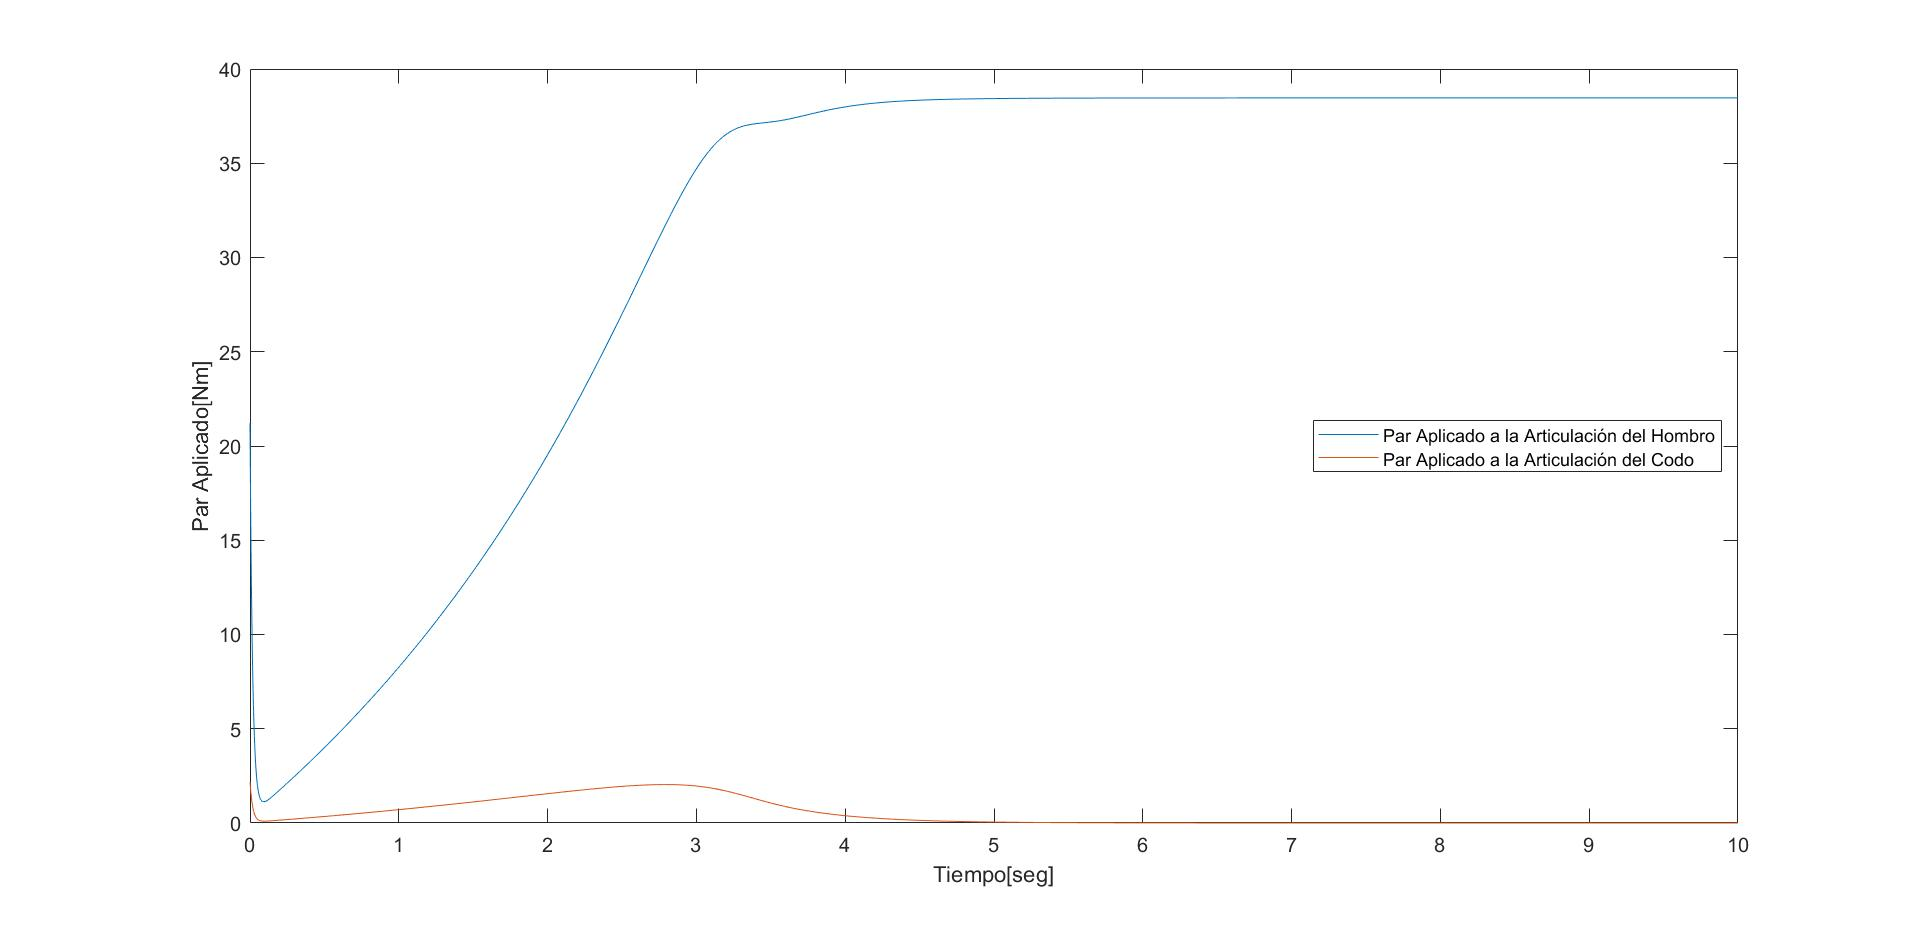
\includegraphics[width=14cm, height=5cm]{IMAGENES/par.jpg}
        \caption{Pares Aplicados en las Articulaciones.}
        \label{fig:par}
    \end{figure}
    
    Se puede observar que los pares aplicados no superan la los valores máximos en ningun instante de la simulación.
    
    \begin{figure}[h]
        \centering
        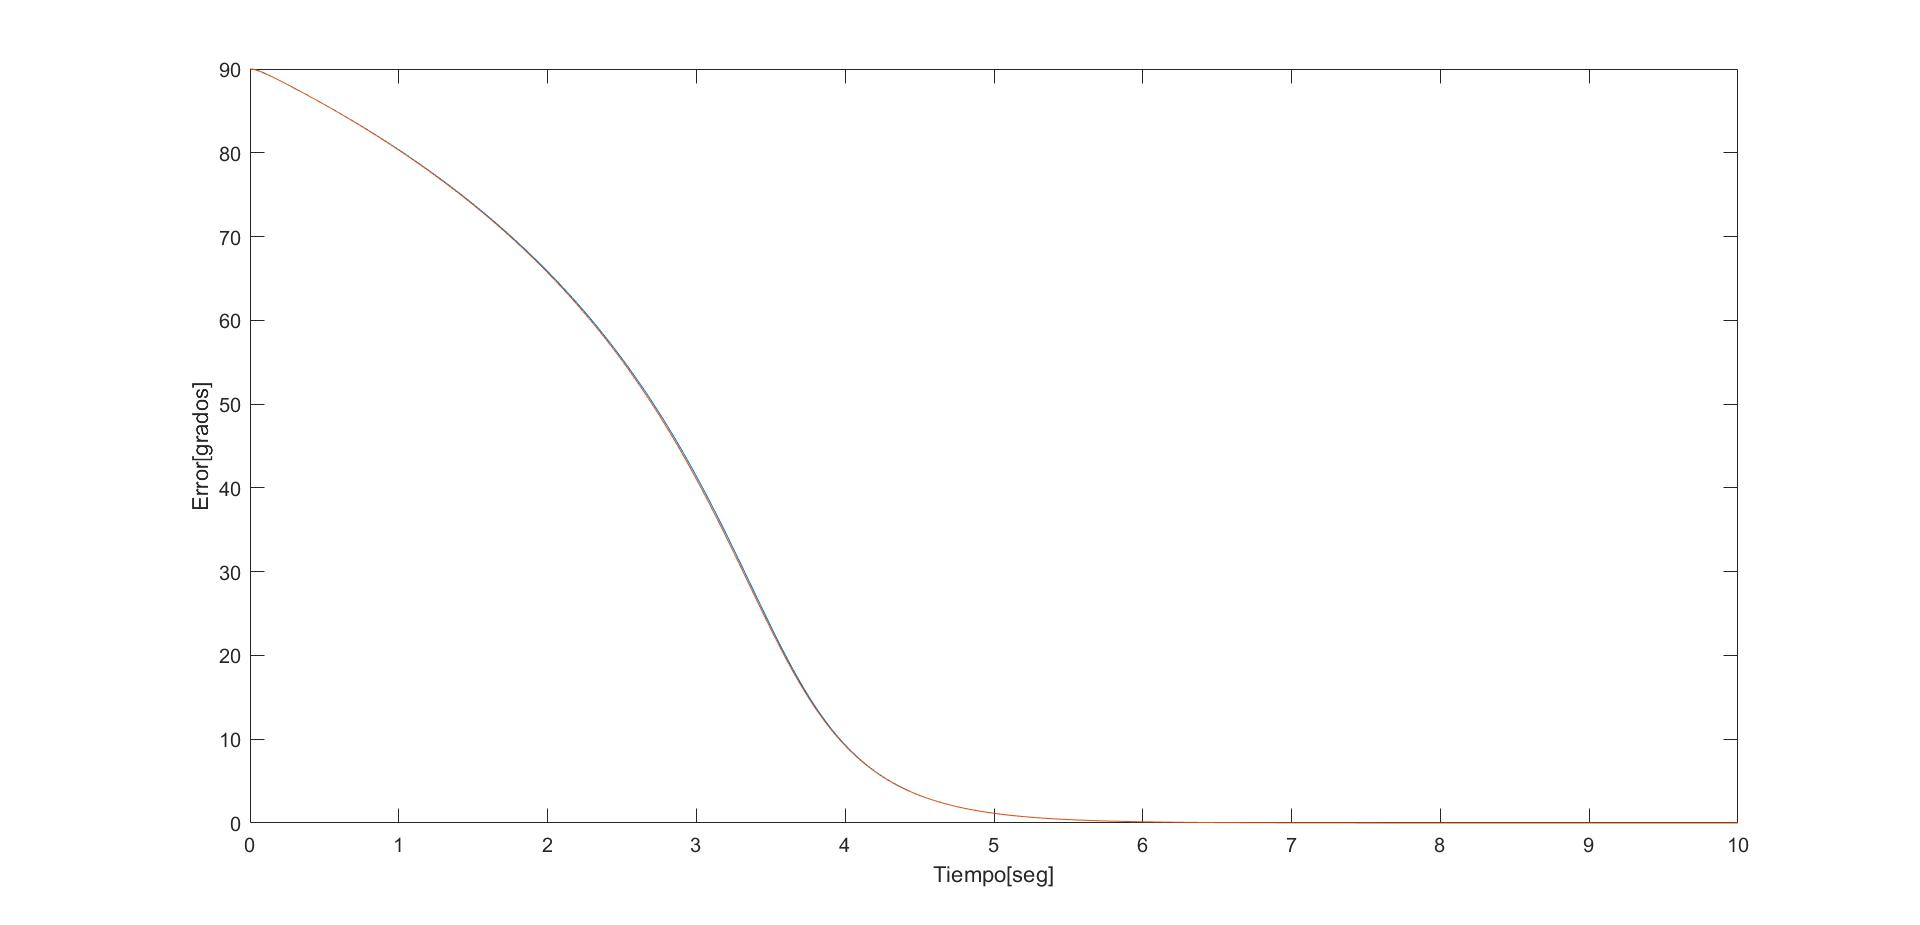
\includegraphics[width=14cm, height=5cm]{IMAGENES/error.jpg}
        \caption{Evolución del Error de Posición en el Tiempo.}
        \label{fig:error}
    \end{figure}

    Como se demostró podemos observar que el error de posición converge asintóticamente a cero según transcurre el tiempo que ya fue atrapado por el atractor del punto de equilibrio[\cite{reyes2011robotica}].
\end{enumerate}
\section{Conclusiones}
Se desarrollaron demostraciones usando un nuevo esquema de control, haciendo uso de la ecuacion en lazo cerrado en conjunto con el modelo dinámico del robot manipulador. En una primera instancia se hizo el tratamiento matemático para uno  de n grados de libertad. Posteriormente se dieron valores numéricos a las matrices de inercia, fricciones, par gravitacional para el caso de un robot manipulador de dos grados de libertad, esto con el objetivo de realizar simulaciones y analizar cualitativamente el comportamiento del algoritmo de control propuesto esto se realizo usando una version en $\mathbb{R}^{2\times2}$ del algoritmo de control cuya existencia de punto de equilibrio ya habia sido demostrada en $\mathbb{R}^{n\times n}$ por lo cual al ser $\mathbb{R}^{2\times2}$ un caso particular, se tenia seguridad de su correcto funcionamiento antes de realizar las simulaciones, este hecho fue comprobado luego de interpretar a los resultados de simulación obtenidos.

\bibliographystyle{apacite}
\bibliography{biblio}
\newpage
\section{Anexos}
Código de simulación principal.
\lstinputlisting[language=matlab]{Matlab/simurobot2gdl.m}
Código de que contiene el modelo dinámico del robot de dos grados de libertad.
\lstinputlisting[language=matlab]{Matlab/robot2gdl.m}
\newpage
Código que contiene el algoritmo de control
\lstinputlisting[language=matlab]{Matlab/alg_control.m}
Gráfica de funciones
\lstinputlisting[language=Python]{IMAGENES/plot.py}
\end{document}
